\documentclass[a4paper]{article}
\usepackage[UTF8]{ctex}
\usepackage{geometry}
\usepackage{graphicx}
\usepackage{url}
\usepackage{multirow}
\usepackage{array}
\usepackage{booktabs}
\usepackage{url}
\usepackage{enumitem}
\usepackage{graphicx}
\usepackage{float}
\usepackage{amssymb}
\usepackage{amsmath}
\usepackage{subfig}
\usepackage{longtable}
\usepackage{pifont}
\usepackage{color}

\allowdisplaybreaks

\geometry{a4paper, scale=0.78}

% \begin{figure}[H]
%     \centering
%     \includegraphics[width=.55\textwidth]{E.png}
%     \caption{矩阵与列向量的乘法}
%     \label{fig:my_label_1}
% \end{figure}

% \left\{
% \begin{array}{ll}
%       x+2x+z=2 & \\
%       3x+8y+z=12 & \\
%       4y+z=2
% \end{array}
% \right.

% \begin{enumerate}[itemindent = 1em, itemsep = 0.4pt, parsep=0.5pt, topsep = 0.5pt]

% \end{enumerate}

%\stackrel{a}{\longrightarrow}

%\underbrace{}_{} %下括号

\title{Expectation Maximization 03  Generalized Expectation Maximization}
\author{Chen Gong}
\date{19 December 2019}

\begin{document}
\maketitle
本小节中,我们想要介绍三个方便的知识点。1. 从狭义的EM算法推广到广义的EM算法;2. 狭义的EM实际上只是广义的EM的一个特例;3. 真正的开始介绍EM算法。

$X$:Observed Variable $\longrightarrow$ $X=\{ x_i \}_{i=1}^N$;

$Z$:Latent Variable $\longrightarrow$ $Z=\{ Z_i \}_{i=1}^N$;

$(X,Z)$:Complete Model;

$\theta$:Model Parameter。

我们希望得到一个参数$\theta$,可以来推导出$X$,也就是$P(X|\theta)$。而这个参数怎么求得呢?所以,这就是一个learning的问题了。

\section{极大似然估计}
所以,根据极大似然估计法的思路,我们要求的最优化参数$\hat{\theta}$为:
\begin{equation}
    \begin{split}
        \hat{\theta} 
        = & \arg\max_{\theta} P(X|\theta) \\
        = & \arg\max_{\theta} \prod_{i=1}^N P(x_i|\theta) \\
        = & \arg\max_{\theta} \sum_{i=1}^N \log P(x_i|\theta)
    \end{split}
\end{equation}

好像,我们这样做就可以解决问题了呀。为什么要多此一举的来引入隐变量$Z$呢?这是因为,我们实际观察的输入空间$\mathcal{X}$的分布$P(X)$,是非常复杂的。可能什么规律都找不出来,这时我们就想到了一个很好的解决办法。我们引入了一个隐变量$Z$,这个变量中包含了我们自己的一些归纳总结,引入了内部结构。而$P(X) = \int_Z P(X,Z)dZ$,实际上就是对$X$进行了分解处理。

\section{广义的EM算法}

EM算法是为了解决参数估计问题,也就是learning问题:
\begin{equation}
    \hat{\theta} = \arg\max_{\theta} P(X|\theta)
\end{equation}

但是,$P(X|\theta)$可能会非常的复杂。那么,在生成模型的思路中,可以假设一个隐变量$Z$。有了这个生成模型的假设以后,我们就可以引入一些潜在归纳出的结构进去。通过$P(X) = \frac{P(X,Z)}{P(Z|X)}$,就可以把问题具体化了。

这里说明一下,我们习惯用的表达是$\log P(X|\theta)$,但是也有的文献中使用$P(X;\theta)$或者$P_\theta(X)$。这三种表达方式代表的意义是等价的。

前面我们已经说过了,我们的目标是:
\begin{equation}
    \log P(X|\theta) = \underbrace{ELBO}_{L(Q,\theta)} + KL(Q||P) \geq L(Q,\theta)
\end{equation}
\begin{equation}
    \left\{
    \begin{array}{ll}
      ELBO = \int_Z Q(Z)\log \frac{P(X,Z|\theta)}{Q(Z)} dZ & \\
      KL(Q||P) = \int_Z Q(Z)\log \frac{Q(Z)}{P(Z|X,\theta)} dZ & \\
    \end{array}
    \right.
\end{equation}

但是,问题马上就上来了,那就是$P(Z|X,\theta)$非常有可能求不出来。那么我们怎么来求解这个方程呢?也就是使下界变得更大。

首先第一步,我们把$\theta$给固定住。那么,$P(Z|X,\theta)$的结果就是一个定值。那么KL越小,ELBO就会越大。由于,$Q(Z)$是我们引入的一个中间变量,那么我们的第一步就是得到:
\begin{equation}
    \hat{Q}(Z) = \arg\min_{Q} KL(Q||P) = \arg\max_Q L(Q,\theta)
\end{equation}

当$Q$被我们求出来以后,我们就可以将$Q$固定了,再来求解$\theta$:
\begin{equation}
    \hat{\theta} = \arg\max_{\theta} L(\hat{q},\theta)
\end{equation}

那么,广义的EM算法,就可以被我们定义为:
\begin{equation}
    \begin{split}
        & E-step:\quad Q^{(t+1)} = \arg\max_{Q} L(Q(Z),\theta^{(t)}) \\
        & M-step:\quad \theta^{(t+1)} = \arg\max_{\theta} L(Q(Z)^{(t+1)},\theta) \\
        & L(Q,\theta) = \mathbb{E}_Q\left[ \log P(X,Z) - \log Q\right]
        = \mathbb{E}_Q\left[ \log P(X,Z) \right] - \mathbb{E}_Q\left[\log Q \right]
    \end{split}
\end{equation}

看到这里,我估计大家已经可以理解上一小节中,为什么有的$\theta$带$(t)$有的不带。因为,首先第一步中是固定$\theta$求$Q$,这里的$\theta$就是来自于上一次迭代的$\theta^{(t+1)}$。第二次,是将上一步求得的$Q$固定,将$\theta$看成参数,来求最优的表达结果的$\theta^{(t+1)}$。另一个方面,从等式(7)的第三行,我们可以可以看出实际上:
\begin{equation}
    ELBO = \mathbb{E}_{Q(Z)}[\log P(X,Z|\theta)] + H(Q(Z))
\end{equation}

我们对比一下上一节讲到的EM算法,就会惊奇的发现,ELBO中最后那个$H(Q(Z))$竟然不见了。这是为什么呢?其实也很好理解的。因为在M-step中,我们假定$Q(Z)$已经是固定的了,那么显然$H[Q(Z)]$就是一个定值了,并且与我们的优化目标$\theta$之间并没有任何的关系,所以就被我们给省略掉了。

所以,本小节中引出了广义EM算法,也说明了原来的EM算法是广义EM算法的一种特殊情况。

\section{坐标上升法}
EM算法的整体描述如下所示:
\begin{equation}
    \left\{
    \begin{array}{ll}
      E-step:\quad Q^{(t+1)} = \arg\max_{Q} L(Q(Z),\theta^{(t)}) & \\
      M-step:\quad \theta^{(t+1)} = \arg\max_{\theta} L(Q(Z)^{(t+1)},\theta) & \\
    \end{array}
    \right.
\end{equation}

这个坐标上升法(SMO)是个什么东西呢?具体的描述,大家可以去网上找找资料看一看。两者都是迭代的思路,在这里我们将它和梯度下降法的优化思路放在一起,做一个小小的对比。大家就会发现有什么不一样的地方,
\begin{figure}[H]
    \centering
    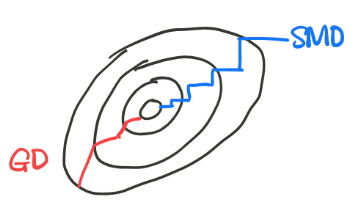
\includegraphics[width=.40\textwidth]{微信图片_20191219100509.png}
    \caption{坐标上升法和梯度上升法的优化思路对比}
    \label{fig:my_label_1}
\end{figure}

我们发现坐标上升法的优化方向基本是恒定不变的,而梯度下降法的优化方向是随着梯度方向而不断发生改变的。

讲到这里,好像一切都很完美,可以圆满的结束了。但是,很不幸的是,问题马上又来了。因为,现实生活中,并没有那么的容易,一切都没有我们想的那么的简单。实际上,有关$P(Z|X,\theta)$的计算,有可能会非常的复杂。所以,我们将采用变分推断(Variable Inference)或者马尔可夫蒙特卡罗采样(Markov Chain Monte Carlo)的方法来求解。结合起来以后就是,VBEM/VEM和MCEM。这里注意一下,Variable Inference和Variable Bayes实际上都是一种东西。

当然,虽然EM算法看上去好像很厉害的样子。但是,没有一种算法可以一劳永逸的解决所有的问题。它一定存在优点,也一定有无法解决的问题。具体描述,大家可以去网上寻找相关的资料,我这里就不做过多的描述了。

\end{document}